\section{HOPG-Probe}\label{sec:hopg-probe}
\subsection*{Struktur}
Hochorientierter pyrolyitscher Graphit (HOPG) ist kristalliner Kohlenstoff, wo Atome einer Schicht
auf einem hexagonalen Gitter geordnet sind, wodurch jedes Atom auf dieser zweidimensionalen
Ebene von drei weiteren Atomen im Winkel von \SI{120}{\degree} verbunden ist. Zwei Schichten
dieses Gitters sind versetzt übereinander geordnet (siehe \cref{fig:hopg-skizze}), weshalb durch die
untere Ebene die Ladungsverteilung auf der Oberfläche beeinflusst wird.\par Wie in
\cref{fig:hopg2} erkennbar ist bei den H-Atomen die Ladungsverteilung minimal und bei A-Atomen maximal.
Die Verteilung bei den B-Atomen befindet sich dazwischen, weshalb diese für das Mikroskop unsichtbar werden,
da ein RTM nicht unmittelbar die Oberflächentopographie messen kann, sondern die Aufenthaltswahrscheinlichkeit der
Elektronen \cite[Kap.1 S.7]{rtm-leitpfaden}.

\begin{figure}[htb]
	\centering
	\begin{subfigure}{0.45\linewidth}
		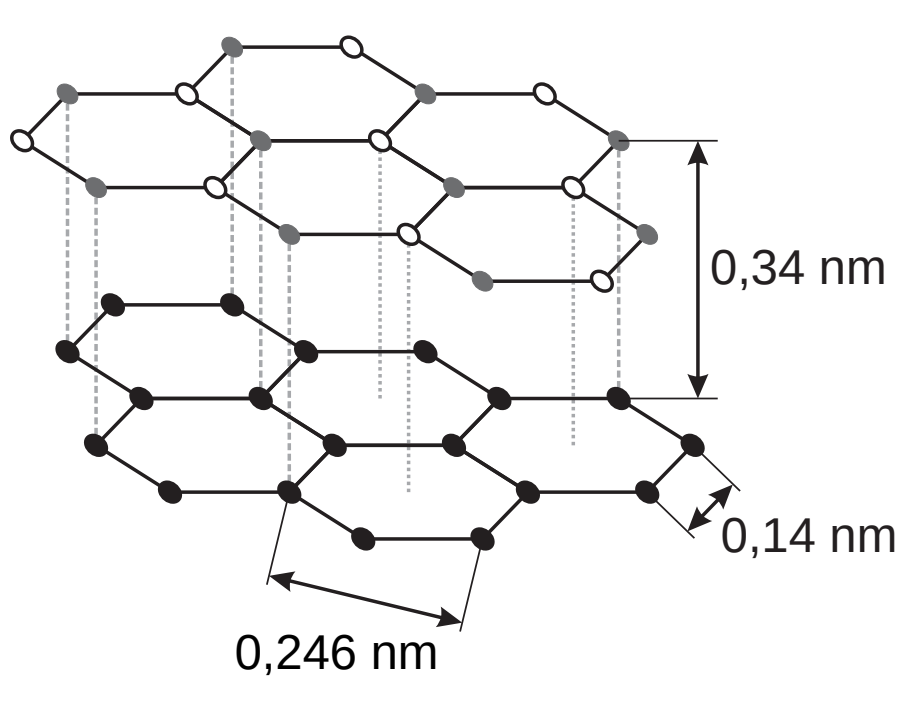
\includegraphics[width=\linewidth]{figs/hopg1.png}
		\caption{Seitenansicht.\cite[S.49]{skript}}
		\label{fig:hopg1}
	\end{subfigure}
	\hspace{0.5cm}
	\begin{subfigure}{0.45\linewidth}
		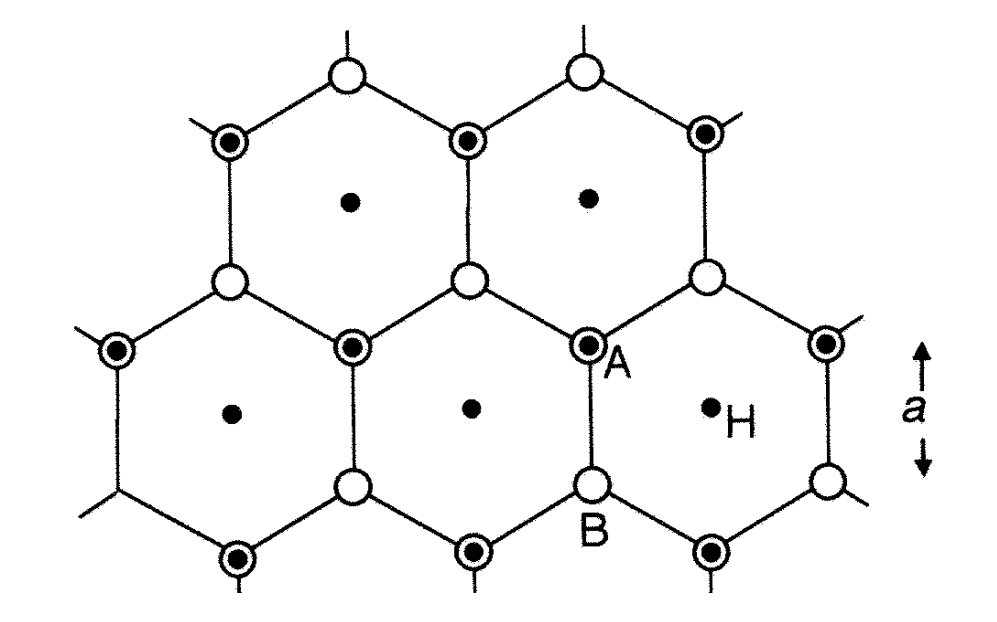
\includegraphics[width=\linewidth]{figs/hopg2.png}
		\caption{Obere Ansicht.\cite[Kap.1 S.17]{rtm-leitpfaden}}
		\label{fig:hopg2}
	\end{subfigure}
	\caption{Hochorientierter pyrolyitscher Graphit.}
	\label{fig:hopg-skizze}
\end{figure}

\subsection*{Vorbereitung}
Im Gegensatz zu Gold wird hier versucht, die atomare Struktur des Graphits aufzulösen.
Dies erfordert hohe Präzision in der Durchführung und der Präparierung der Spitze. Der Platin-Iridium Draht
vor der Rasterung ist in \cref{fig:spitze_hopg_vorher_v2} abgebildet. Vorne ist eine dünne Spitze zur ekennen,
die sich für die Durchführung eignen sollte.

\begin{figure}[htb]
	\centering
	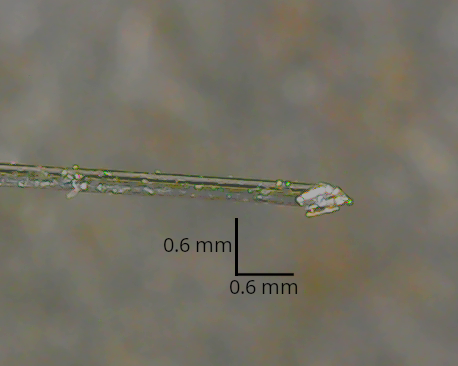
\includegraphics[width=0.5\linewidth]{figs/spitze_hopg_vorher_v2.png}
	\caption{Platin-Iridium Spitze vor Rasterung des HOPG.}
	\label{fig:spitze_hopg_vorher_v2}
\end{figure}

Die Graphit-Probe ist in \cref{fig:usb_mikroskop_hopg} mit zwei unterschiedlichen
Vergrößerungen abgebildet. Zu erkennen ist eine Stufenstruktur auf der Obefläche, die jedoch
deutlich größer ist als die Fläche, die gerastert werden soll. Daher kann mit dieser
Probe gearbeitet werden.


\begin{figure}[htb]
	\centering
	\begin{subfigure}{0.45\linewidth}
		\centering
		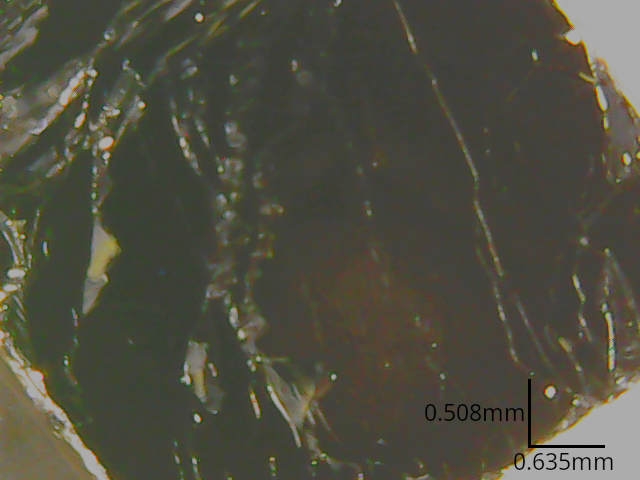
\includegraphics[width=\linewidth]{figs/hopg_skala1.png}
		\caption{Skala 1}
		\label{fig:hopg_skala1}
	\end{subfigure}
	\hspace{0.5cm}
	\begin{subfigure}{0.45\linewidth}
		\centering
		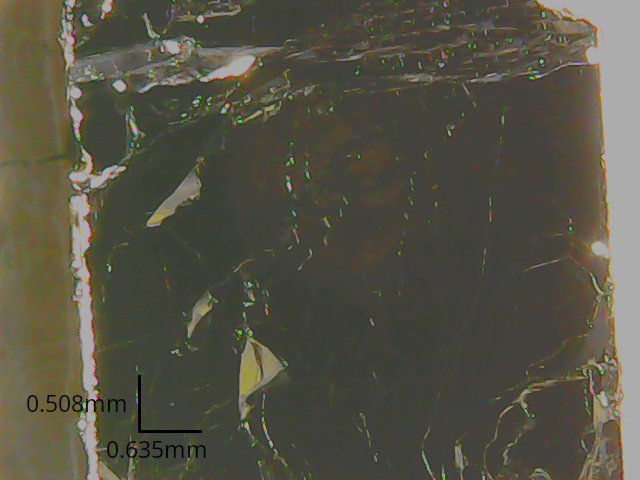
\includegraphics[width=\linewidth]{figs/hopg_skala2.png}
		\caption{Skala 2}
		\label{fig:hopg_skala2}
	\end{subfigure}
	\caption{USB-Mikroskop Aufnahmen von HOPG nach Abziehen der obersten Schicht.}
	\label{fig:usb_mikroskop_hopg}
\end{figure}

\subsection*{Auswertung}

Nach erfolgreicher Annäherung der Probe an die Spitze wird zunächst ein Bild
mit einer großen Breite gemacht, um die Grobstruktur der Oberfläche
zu bekommen um damit einen ausreichend flachen Flächenabschnitt
finden zu können. Ein Bild bei einer Breite von $\SI{200}{\nm}$ ist in 
\cref{fig:hopg_rtm_weitaufnahme} zu sehen, wobei das oben rechte Viertel 
von einer flachen Ebene gefüllt wird, wo die Höhe nur um einen Atomdurchmesser schwankt.

\begin{figure}[htb]
	\centering
	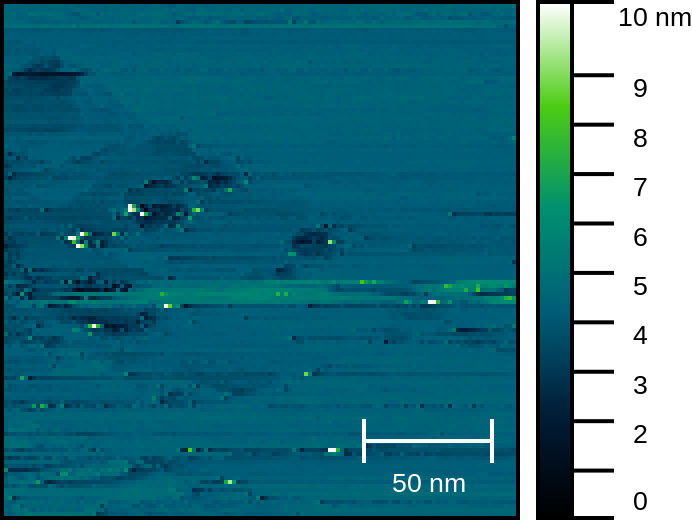
\includegraphics[width=0.6\linewidth]{figs/HOPG10558.png}
	\caption{$I_\mathrm{set}=\SI{5}{\nm}$, $V=\SI{500}{\milli\volt}$, $P=1000$, $I=2000$,
		$v=\SI{1}{\nm\per\s}$}
	\label{fig:hopg_rtm_weitaufnahme}
\end{figure}

